\documentclass[a4paper,11pt]{article}
\usepackage{amsmath,amsthm,amsfonts,amssymb,amscd,amstext,vmargin,graphics,graphicx,tabularx,multicol} 
\usepackage[francais]{babel}
\usepackage[utf8]{inputenc}  
\usepackage[T1]{fontenc} 
\usepackage{pstricks-add,tikz,tkz-tab,variations}
\usepackage[autolanguage,np]{numprint} 
\usepackage{color}

\setmarginsrb{1.5cm}{0.5cm}{1cm}{0.5cm}{0cm}{0cm}{0cm}{0cm} %Gauche, haut, droite, haut
\newcounter{numexo}
\newcommand{\exo}[1]{\stepcounter{numexo}\noindent{\bf Exercice~\thenumexo} : \marginpar{\hfill /#1}}
\reversemarginpar


\newcounter{enumtabi}
\newcounter{enumtaba}
\newcommand{\q}{\stepcounter{enumtabi} \theenumtabi.  }
\newcommand{\qa}{\stepcounter{enumtaba} (\alph{enumtaba}) }
\newcommand{\initq}{\setcounter{enumtabi}{0}}
\newcommand{\initqa}{\setcounter{enumtaba}{0}}

\newcommand{\be}{\begin{enumerate}}
\newcommand{\ee}{\end{enumerate}}
\newcommand{\bi}{\begin{itemize}}
\newcommand{\ei}{\end{itemize}}
\newcommand{\bp}{\begin{pspicture*}}
\newcommand{\ep}{\end{pspicture*}}
\newcommand{\bt}{\begin{tabular}}
\newcommand{\et}{\end{tabular}}
\renewcommand{\tabularxcolumn}[1]{>{\centering}m{#1}} %(colonne m{} centrée, au lieu de p par défault) 
\newcommand{\tnl}{\tabularnewline}

\newcommand{\bmul}[1]{\begin{multicols}{#1}}
\newcommand{\emul}{\end{multicols}}

\newcommand{\trait}{\noindent \rule{\linewidth}{0.2mm}}
\newcommand{\hs}[1]{\hspace{#1}}
\newcommand{\vs}[1]{\vspace{#1}}

\newcommand{\N}{\mathbb{N}}
\newcommand{\Z}{\mathbb{Z}}
\newcommand{\R}{\mathbb{R}}
\newcommand{\C}{\mathbb{C}}
\newcommand{\Dcal}{\mathcal{D}}
\newcommand{\Ccal}{\mathcal{C}}
\newcommand{\mc}{\mathcal}

\newcommand{\vect}[1]{\overrightarrow{#1}}
\newcommand{\ds}{\displaystyle}
\newcommand{\eq}{\quad \Leftrightarrow \quad}
\newcommand{\vecti}{\vec{\imath}}
\newcommand{\vectj}{\vec{\jmath}}
\newcommand{\Oij}{(O;\vec{\imath}, \vec{\jmath})}
\newcommand{\OIJ}{(O;I,J)}


\newcommand{\reponse}[1][1]{%
\multido{}{#1}{\makebox[\linewidth]{\rule[0pt]{0pt}{20pt}\dotfill}
}}

\newcommand{\titre}[5] 
% #1: titre #2: haut gauche #3: bas gauche #4: haut droite #5: bas droite
{
\noindent #2 \hfill #4 \\
#3 \hfill #5

\vspace{-1.6cm}

\begin{center}\rule{6cm}{0.5mm}\end{center}
\vspace{0.2cm}
\begin{center}{\large{\textbf{#1}}}\end{center}
\begin{center}\rule{6cm}{0.5mm}\end{center}
}



\begin{document}
\pagestyle{empty}
\titre{Contrôle - Théorème de Thalès et sa réciproque}{Nom :}{Prénom :}{Classe}{Date}
\vspace*{0.5cm}


\exo{3} QCM : Entourer \textbf{la} bonne réponse.


\renewcommand{\arraystretch}{3}
\begin{flushleft}

\begin{tabular}{|c|p{4.7cm}|c|c|c|}
\hline 
 &  & \textbf{REPONSE A} & \textbf{REPONSE B }& \textbf{REPONSE C} \\ 
\hline 
\textbf{FIGURE 1} & \includegraphics[scale=1]{qcm1.eps} \textbf{Quelle est la bonne égalité ?}  & $\dfrac{AD}{AC}=\dfrac{AB}{DE}=\dfrac{BE}{BC}$ & $\dfrac{CD}{DA}=\dfrac{CE}{EB}=\dfrac{DE}{AB}$ &  $\dfrac{CD}{AC}=\dfrac{CE}{CB}=\dfrac{DE}{AB}$   \\ 
\hline 
\textbf{FIGURE 2} &  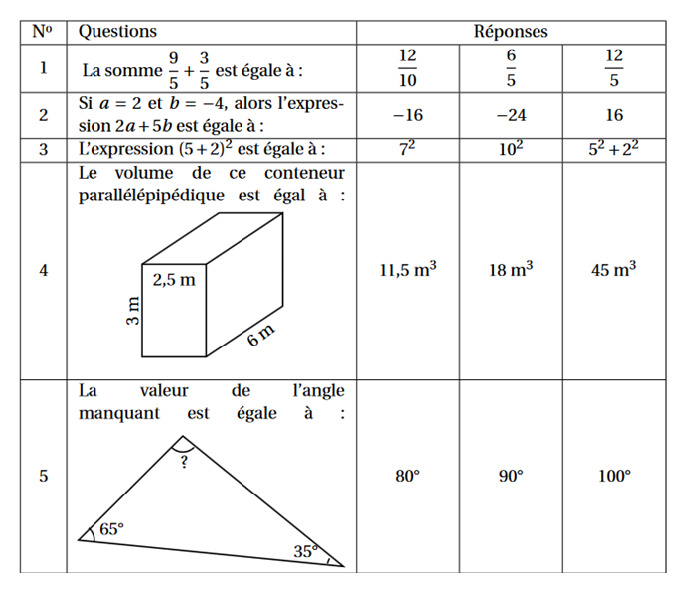
\includegraphics[scale=1]{qcm2.eps} \textbf{Quelle est la bonne égalité ?} &$\dfrac{AC}{CD}=\dfrac{BC}{CE}=\dfrac{AB}{DE}$  & $\dfrac{EC}{CB}=\dfrac{DC}{CA}=\dfrac{AB}{DE}$ & $\dfrac{AC}{AD}=\dfrac{BC}{BE}=\dfrac{AB}{DE}$\\ 
\hline 
\textbf{FIGURE 3} & \includegraphics[scale=1.1]{qcm3.eps} \textbf{Les droites (BE) et (FC) sont-elles parallèles ?} & Non & Oui & On ne peut pas savoir \\ 
\hline 
\end{tabular} 
\end{flushleft}

\vspace*{0.5cm}

\exo{3} Pour mesurer la hauteur de sa maison, Laurent vise le sommet de son toit et fait coïncider avec le haut de
son muret. Voici un schéma de la situation:

\begin{center}
\includegraphics[scale=0.9]{thalesbrevet2.eps} 
\end{center}

Le muret a une hauteur de 1,30 m. Laurent (L) est à 4 m du muret et la distance entre le centre de la maison
et le muret est de 21 m.\\
 	
$\rightarrow$ \textbf{ Déterminer la hauteur de la maison.}\\
\newpage
\vspace*{0.5cm}
\exo{4} La figure n'est pas faite en vraie grandeur.	
\bmul{2}			    
	
Pour la figure ci-contre, on sait que :	\\
- Les droites (BC) et (DF) sont parallèles, 	\\			       
- AC = 18 cm ;  CG = 9 cm ;  GE = 15 cm  et  EF = 22,5 cm.		\\

$\rightarrow$	\textbf{Calculer la longueur BC.}\\
\textit{ (Pour bien repérer dans quels triangles vous travaillez, n'hésitez pas à mettre de la couleur et écrire les mesures que vous connaissez.)}\\

\columnbreak

\includegraphics[scale=0.65]{thalesenonce.eps} 

\emul

\vspace*{0.5cm}


\exo{4}  Le dessin ci-dessous est un schéma d'une table à repasser en centimètres.

\begin{center}
\includegraphics[scale=0.8]{thales7.eps} 
\end{center}

$\rightarrow$ \textbf{Cette table à repasser est-elle parallèle au sol ? Justifier votre réponse.}\\


\vspace*{0.5cm}

\exo{6} 
Des élèves participent à une course à pied.\\
Avant l'épreuve, un plan leur a été remis.
Il est représenté par la figure ci-contre.\\
On convient que :\\
- Les droites (AE) et (BD) se coupent en C.\\
- Les droites (AB) et (DE) sont parallèles.\\
- ABC est un triangle rectangle en A.

\begin{center}
\includegraphics[scale=0.6]{thalesbrevet.eps} 
\end{center}

$\rightarrow$ \textbf{ Calculer la longueur réelle du parcours ABCDE.}\\
\textit{Si le travail n'est pas terminé, laisser tout de même une trace de la recherche.\\ Elle sera
prise en compte dans la notation.}




\end{document}
